\section{Régression linéaire régularisée}

\begin{figure}[!h]
    \begin{minipage}{.48\linewidth}
        Nous avons déjà appliqué la régression linéaire dans le \textit{TP1}, le principe sera le même, mais cette fois-ci nous 
        allons appliquer le principe de régularisation rencontré dans le \textit{TP2} pour la régression logistique. L'objectif 
        est de prédire la quantité d'eau qui s'écoule d'un barrage à l'aide de la variation du niveau d'eau dans un réservoir.\\

        Pour rappel, l'hypothèse dans le cas d'une régression linéaire est la suivante~:
        \begin{equation}\label{eq:regression_linear}
            h_\theta(x) = x^T \theta =\theta_0 + \theta_1 x_1
        \end{equation}

    \end{minipage}\hfill
    \begin{minipage}{.48\linewidth}
        \begin{center}
            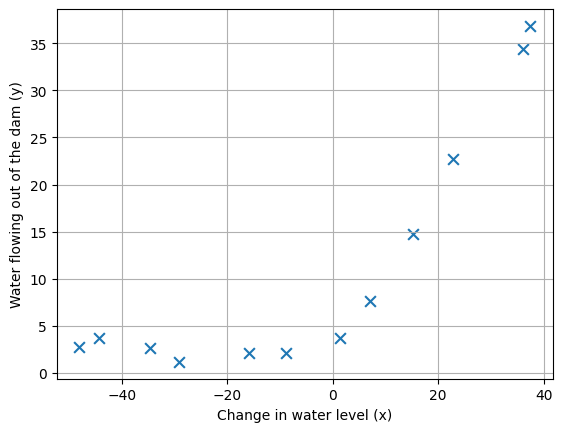
\includegraphics[width=0.9\textwidth]{./img/3.1.png}
            \caption{\label{fig:data-plot}Visualisation du jeu de données}  
        \end{center}
    \end{minipage}
\end{figure}


\subsection{Fonction de coût $J(\theta)$ régularisée}


\begin{equation}\label{eq:cout-reg}
    J(\theta) = \frac{1}{2m} \sum_{i=1}^{m}(h_\theta(x^{(i)}) - y^{(i)})^2 + \underbrace{\frac{\lambda}{2m} \left[\sum_{j=1}^{n} \theta_j^2\right]}_{(a)}
 \end{equation} 

\begin{itemize}
    \item [(a)] La régularisation nous permet d'atténuer tous les coefficients $\theta$ en fonction du paramètre $\lambda$. Plus celui-ci est petit, plus $\theta$ sera atténué.
\end{itemize}

\begin{figure}[!h]
\begin{minted}[frame=lines, framesep=2mm, baselinestretch=1.2, fontsize=\footnotesize, linenos, breaklines=true]{python}
def linearRegCostFunction(X, y, theta, Lambda):
    m,n = X.shape 
    theta = theta.reshape((n,1)) 
    h = X @ theta
    J = (1/(2*m)) * np.sum((h - y) ** 2) + (Lambda/(2*m)) * np.sum(theta[1:] ** 2)

    return J.flatten()

""" output
Cost at theta = [1  1]: 303.993192 
(this value should be about 303.993192)
"""
\end{minted}   
\captionof{listing}{Fonction linearRegCostFunction}
\end{figure}




\subsection{Descente de gradient régularisée}
\begin{align}\label{eq:descente-gradient-reg}
    \frac{\partial J(\theta)}{\partial \theta_j} = \frac{1}{m} \sum_{i=0}^{m} (h_\theta(x^{(i)}) - y^{(i)}) x_j^{(i)} \qquad \qquad \qquad \text{pour} \quad j=0 \\
    \frac{\partial J(\theta)}{\partial \theta_j} = \frac{1}{m} \left[ \sum_{i=0}^{m} (h_\theta(x^{(i)}) - y^{(i)}) x_j^{(i)} + \underbrace{\lambda \theta_j}_{(a)} \right] \qquad \qquad \qquad \text{pour} \quad j\geq1 \nonumber
\end{align}

\begin{itemize}
    \item [(a)] Ici, on adapte également la régularisation sur la descente de gradient comme pour le coût $J(\theta)$. Conventionnellement on ne régularise pas $\theta_0$
    puisqu'il s'agit du biais.
\end{itemize}

\vspace{0.5cm}


Le calcul du coût $J(\theta)$ permet de mesurer la qualité de la prédiction, si le coût est faible alors notre prédiction est proche des valeurs réelles et inversement si le coût est important. \\
On remarque ici avec l'équation \ref{eq:cout-reg} qui utilise l'équation \ref{eq:regression_linear}, que les seules valeurs qui puissent influencer notre coût est $\theta$ et $\lambda$. Pour réduire notre coût, nous devons donc minimiser $\theta$, c'est l'objectif
de la descente de gradient, minimiser $J(\theta)$.

\vspace{0.2cm}

\begin{figure}[!h]
\begin{minted}[frame=lines, framesep=2mm, baselinestretch=1.2, fontsize=\footnotesize, linenos, breaklines=true]{python}
def linearRegCostFunction(X, y, theta, Lambda):
    m,n = X.shape # number of training examples
    theta = theta.reshape((n,1)) # in case where theta is a vector (n,) 
    h = X @ theta
    J = (1/(2*m)) * np.sum((h - y) ** 2) + (Lambda/(2*m)) * np.sum(theta[1:] ** 2)
    grad = (1/m) * (X.T @ (h - y))
    grad[1:] += (Lambda/m * theta[1:])

    return J.flatten(), grad.flatten()
""" output
Gradient at theta = [1  1]:  [-15.303016 598.250744] 
(this value should be about [-15.303016 598.250744])
"""
\end{minted}   
\captionof{listing}{\label{lst:linearRegCostFunction}Fonction linearRegCostFunction}
\end{figure}




\subsection{Visualisation de la régression linéaire régularisée}

\begin{figure}[!h]
    \begin{minipage}{.48\linewidth}
        À l'aide de la fonction \textit{trainLinearReg} qui utilise elle-même notre fonction \ref{lst:linearRegCostFunction} nous pouvons calculer les valeurs optimales de $\theta$. \\
        On constate que notre régression n'est pas optimale, on peut même dire que nous sommes en sous-apprentissage. \\
        Le problème ne vient pas de $\lambda$ étant donné qu'il vaut 0, la régularisation n'a donc aucune utilité. 
        Si nous obtenons un résultat similaire c'est dû aux nombres insuffisants de caractéristiques, notre $\theta$ est seulement de dimension~2. Pour résoudre ce problème, nous pouvons modifier nos caractéristiques sous forme polynomiale, cette méthode sera appliquée plus tard.
    \end{minipage}\hfill
    \begin{minipage}{.48\linewidth}
        \begin{center}
            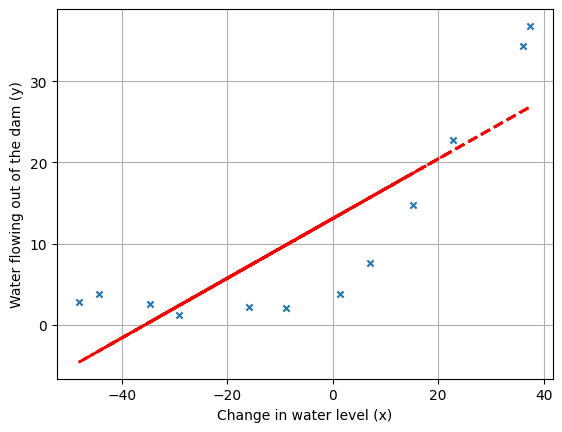
\includegraphics[width=0.9\textwidth]{./img/3.4.png}
            \caption{\label{fig:reg-lin-plot}Régression linéaire régularisée}  
        \end{center}
    \end{minipage}
\end{figure}
